\documentclass[parskip=half]{scrartcl}
\usepackage{amsmath}
\usepackage[T1]{fontenc}
\usepackage{gensymb}
\usepackage{graphicx}

\usepackage{natbib}

\bibliographystyle{gi-nsf}
\newcommand{\changefont}[3]{\fontfamily{#1} \fontseries{#2} \fontshape{#3} \selectfont}

%% commands to facilitate units and temperature
\newcommand{\unit}[1]{\ensuremath{\,\mathrm{#1}}}
\newcommand{\s}[1]{\ensuremath{\,\mathrm{#1}}}
\newcommand{\cels}[1]{\ensuremath{#1^{\circ}\,\mathrm{C}}}


% ---------------------------------------------------------------------------------------
% definition of header and footer
% ---------------------------------------------------------------------------------------

\usepackage[automark,headsepline,footsepline]{scrlayer-scrpage}
\clearscrheadings	
\ihead{Thermodynamics of glaciers}
\ohead{McCarthy Summer School 2024}
\cfoot{\pagemark}
\setkomafont{pagehead}{\normalfont}	
\setkomafont{pagenumber}{\normalfont\rmfamily}




% ---------------------------------------------------------------------------------------
% Koma-Script - Settings
% ---------------------------------------------------------------------------------------
\addtokomafont{caption}{\small}
\setkomafont{captionlabel}{\sffamily\bfseries}
% \setkomafont{caption}{\sffamily}
\setcapindent{1em}

\pagestyle{scrheadings}


\begin{document}

\vspace{-5em}

\title{Thermodynamics of Glaciers \\[.2em]
\rule[1em]{\textwidth}{2pt}
\LARGE\textsf{Exercise}
}
\date{}

\vspace{-5em}

\maketitle


\vspace{-5em}


\section{Climate history}

Air temperatures in Alaska was oscillating with a period of about 50 years and an amplitude of about 2$\,^\circ\text{C}$ between 1950 and 2000. 

\paragraph{Question} How deep down would you be able to detect such temperature variation in stagnant ice if the accuracy of your temperature sensors are 0.02$\,\mathrm{K}$ assuming an ice temperature of $-\cels{3}$?

\section{Cold content}

Carl decided that snow is much more interesting than glacier ice. On a sunny morning in late March somewhere outside of Fairbanks, he measures the temperature profile in the snow pack after a cold night (Figure~\ref{fig:snow-temp-profile}). During the day air temperatures increase above the freezing point and it starts raining. The cold content can be eliminated by release of energy from refreezing water. 

\paragraph{Question} How much melt in mm\,w.e. (water equivalent) or kg/m$^{2}$ is needed to completely eliminate the cold content? Hint: Make a reasonable guess for an anverage snow density.

\begin{figure}
  \centering
  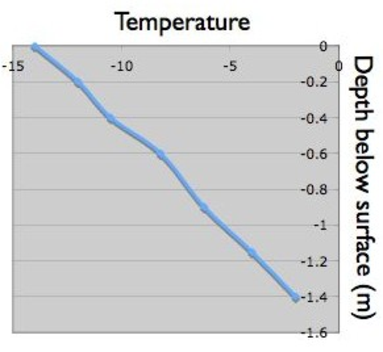
\includegraphics[width=10cm]{figures/cold-content} 
  \caption{Snow temperature profile}
  \label{fig:snow-temp-profile}
\end{figure}

\section{Melting temperature depression}

What is the pressure melting temperature at the base of Gornergletscher (Figure~\ref{fig:temp-profile-gorner})? What does the Clausius-Clapeyron relation indicate in terms of air-saturation of the meltwater? The pressure $p$ is the sum of the hydrostatic pressure and the atmospheric pressure, $p = \rho g H + p_{\mathrm{atm}}$. Assume $p_{\mathrm{atm}} = 75\,\mathrm{kPa}$.

\begin{figure}[tbhp]
 \centering
 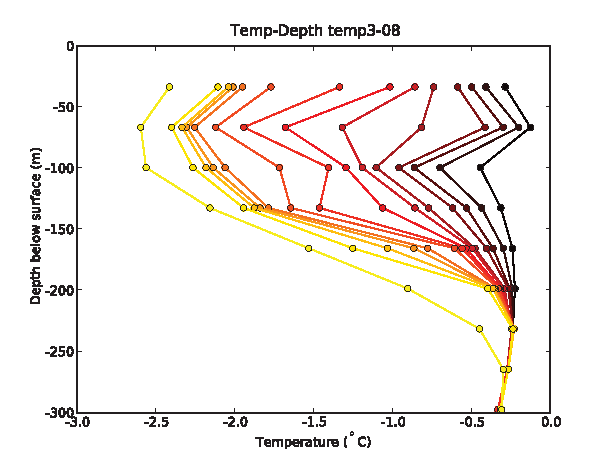
\includegraphics[width=0.6\textwidth]{figures/gorner-temp-depth_temp3-08} 
 \caption{Cooling of a borehole drilled in the confluence area of
   Gorner-/Grenzgletscher. Temperatures  measured every day after
   completion of drilling are shown in increasingly lighter colors, and after three months
   (leftmost yellow curve). Data from \cite{Ryser2009}.
   \label{fig:temp-profile-gorner}}
\end{figure}
\section{Lake Vostok}

\begin{enumerate}
\item Describe 2 different ways how heat can be moved through a polar ice sheet.
\item What is the P\'eclet Number, and how is it useful?
\item The coldest temperature ever recorded is -\cels{89} at Vostok in East Antarctica (in July 1983). The mean annual temperature is -\cels{55}. However, deep under the ice is lake Vostok, a lake of the size of lake Ontario. Calculate the minimum geothermal flux needed for a lake to form. Possibly relevant quantities:
  \begin{itemize}
  \item Surface elevation $3488\,\mathrm{m}$
  \item Ice thickness $3300\,\mathrm{m}$
  \item Snow accumulation rate $2\,\mathrm{cm}\,\mathrm{a}^{-1}$ (water equivalent)
  \item A reasonable average thermal conductivity for the cold temperatures of the East Antarctic Ice Sheet is $k = 2.5\,\mathrm{W}\,\mathrm{m}^{-1}\,\mathrm{K}^{-1}$.
  \end{itemize}
\end{enumerate}


\bibliography{thermobib}
\end{document}
